\documentclass{article}

% Paquete para establecer los márgenes de la página
\usepackage[top=1cm, bottom=1cm, left=2cm, right=2cm]{geometry}
\newif\ifincludeimages
\includeimagestrue % Include images by default

% Paquete para mejorar el manejo de fuentes
\usepackage[T1]{fontenc}
\usepackage[utf8]{inputenc}
\usepackage{lmodern}
\usepackage{qrcode}
\usepackage{xcolor}
\usepackage{titlesec}
\usepackage{svg}
\titleformat{\section}{\large\bfseries}{\thesection}{1em}{}

% Paquete para personalizar listas con viñetas
\usepackage{enumitem}
\setlist[itemize]{leftmargin=*}
\usepackage[colorlinks=true, citecolor={red!70!black}, linkcolor={red!40!black}, urlcolor={blue!40!black}, pdfborder={0 0 0}]{hyperref}

% Paquete para incluir imágenes
\usepackage{graphicx}
\usepackage{multicol}

\begin{document}

\pagestyle{empty} % Eliminar números de página

% Sección del encabezado con imagen
\begin{center}
\begin{minipage}[t]{0.2\textwidth}
\vspace{0pt}

\includegraphics[width=3cm]{img.png}
\end{minipage}
\hspace{1cm}
\begin{minipage}[t]{0.7\textwidth}
\vspace{0pt}
\textbf{CURRICULUM VITAE}\\
\textbf{Nombre:} Lic. Javier Alejandro Oramas López\\
\\
\textbf{Teléfono:} +53 59334374 \\
\textbf{Correo electrónico:} javiale2000@gmail.com \\
\textbf{Fecha de nacimiento:} 02/25/2000\\
\textbf{github:} \href{https://github.com/JavierOramas}{JavierOramas} \\
\textbf{linkedin:} \href{https://www.linkedin.com/in/javier-alejandro-oramas-l%C3%B3pez-7ab47b160/}{javier-alejandro-oramas} \\
\end{minipage}
\end{center}

\section*{Experiencia}
    \textbf{Profesor Adiestrado (Redes de Computadoras)} \hfill desde\textbf{01/2024}\\ 
    MATCOM, UH
    \href{matcom.uh.cu}{MATCOM}\\
    Profesor adistrado en la Carrera de Ciencia de la Computación\\
    \vspace{0.1cm}\\
    \textbf{Desarrollador Backend} \hfill desde\textbf{10/2023}\\ 
    Fonoma Cuba, (remoto)
    \href{fonoma.com}{Fonoma}\\
    Desarrollo Backend en django, fastapi y nodejs, unit test y DevOps\\
    \vspace{0.1cm}\\
    \textbf{Desarrollador} \hfill \textbf{05/2021 - 10/2024}\\ 
    American Behavioral Solutions, Arizona (remoto)
    \href{americanbehavioralsolutions.com}{ABS}\\
    Desarrollo y despliegue de un sistema de gestión de supervisiones\\

% Sección de educación
\section*{Educación}
\textbf{Licenciado en Ciencias de la Computación} \hfill  \textbf{2018-2024}\\
\href{https://matcom.in/}{MATCOM}, \href{https://uh.cu}{Universidad de La Habana}, Cuba\\
\vspace{0.1cm}\\
\textbf{Becario de Investgaci\'on (IA)} \hfill \textbf{2023-2024}\\
\href{https://matcom.in/}{MATCOM}, \href{https://uh.cu}{Universidad de La Habana}, Cuba\\
\href{https://www.colmex.mx/}{El Colegio de M\'exico}, CDMX, M\'exico\\
\vspace{0.1cm}\\
\textbf{\hyperref[sec:bachelor]{Bachiller en Ciencias}} \hfill \textbf{2015-2018}\\
Instituto Vocacional de Ciencias Exactas Ernesto Guevara, Cuba

\section*{Proyectos Personales}
\begin{minipage}{0.8\textwidth}
\parbox{0.8\linewidth}{\textbf{Sistema de archivos distribuido para \href{https://autogoal.github.io/}{AutoGOAL}}}\hfill \textbf{06/2023} \\
Proyecto Académico\\
(descubrimiento automático, tolerancia a fallas, replicación)\\
\href{https://github.com/geeksLabTech/kade-drive}{ver código}\\
\end{minipage} \hfill \qrcode[height=0.6in]{https://github.com/geeksLabTech/kade-drive}\\\\
\begin{minipage}{0.8\textwidth}
\parbox{0.8\linewidth}{\textbf{Modelo para inferir la matriz de contactos de Cuba utilizando Aprendizaje Automático}} \hfill \textbf{06/2023}\\
Proyecto Académico\\
\href{https://github.com/geeksLabTech/epidemic-classification-ml-project}{ver código}\\
\end{minipage} \hfill \qrcode[height=0.6in]{https://github.com/geeksLabTech/epidemic-classification-ml-project}\\\\
\begin{minipage}{0.8\textwidth}
\parbox{0.8\linewidth}{\textbf{DSL para el lenguaje de Michaelson}} \hfill \textbf{01/2023}\\
Proyecto Académico\\
Análisis sintáctico, léxico, comprobación de sintaxis y semántica.\\
\href{https://github.com/geeksLabTech/compilation-dsl-project}{ver código}\\
\end{minipage} \hfill \qrcode[height=0.6in]{https://github.com/geeksLabTech/compilation-dsl-project}\\\\
\begin{minipage}{0.8\textwidth}
\parbox{0.8\linewidth}{\textbf{Predicción de la Copa Mundial de la FIFA utilizando planificación de IA y simulación basada en agentes impulsada por datos}} \hfill \textbf{12/2023}\
Proyecto Académico\
\href{https://github.com/geeksLabTech/FIFA_World_Cup_2022}{ver código}\\
\end{minipage} \hfill \qrcode[height=0.6in]{https://github.com/geeksLabTech/FIFA_World_Cup_2022}\\\\
\begin{minipage}{0.8\textwidth}
\parbox{0.8\linewidth}{\textbf{Desarrollo de un servidor web en C para Linux}} \hfill \textbf{01/2022}\\
Proyecto Académico\\
\href{https://github.com/geeksLabTech/web_server}{ver código}\\
\end{minipage} \hfill \qrcode[height=0.6in]{https://github.com/geeksLabTech/web_server}\\\\
\begin{minipage}{0.8\textwidth}
    \parbox{0.8\linewidth}{\textbf{Desarrollo de una Shell de Linux en C}} \hfill \textbf{12/2021}\\
    Proyecto académico\\
    \href{https://github.com/geeksLabTech/SO_Shell}{ver código}\\
    \end{minipage} \hfill \qrcode[height=0.6in]{https://github.com/geeksLabTech/SO_Shell}\\\\
    \begin{minipage}{0.8\textwidth}
    \parbox{0.8\linewidth}{\textbf{Desarrollo de un Microprocesador MIPS Funcional}} \hfill \textbf{06/2021}\\
    Proyecto académico\\
    \href{https://github.com/JavierOramas/MIPS-Micro/blob/master/informe.pdf}{ver informe}\\
    \href{https://github.com/JavierOramas/MIPS-Micro}{ver código}\\
    \end{minipage} \hfill \qrcode[height=0.6in]{https://github.com/JavierOramas/MIPS-Micro}\\\\
    \begin{minipage}{0.8\textwidth}
    \parbox{0.8\linewidth}{\textbf{Juego de TicTacToe utilizando el algoritmo Minimax en Python}} \hfill \textbf{05/2021}\\
    Proyecto académico\\
    \href{https://github.com/JavierOramas/TicTacToe_AI}{ver código}\\
    \end{minipage} \hfill \qrcode[height=0.6in]{https://github.com/JavierOramas/TicTacToe_AI}\\\\
    \begin{minipage}{0.8\textwidth}
    \parbox{0.8\linewidth}{\textbf{Desarrollo de un Bot para automatizar preguntas frecuentes con una base de conocimientos para un sitio web}} \hfill \textbf{04/2021}\\
    Proyecto académico\\
    Producto escalar euclidiano\\
    \href{https://github.com/JavierOramas/FAQ-Chat-Bot-Nous}{ver código}\\
    \end{minipage} \hfill \qrcode[height=0.6in]{https://github.com/JavierOramas/FAQ-Chat-Bot-Nous}\\\\
    \begin{minipage}{0.8\textwidth}
    \parbox{0.8\linewidth}{\textbf{Desarrollo de la aplicación \hyperref[sec:laluu]{LaLuu} para estimar el consumo de energía basado en los dispositivos y su tiempo de uso,}} \hfill \textbf{01/2021}\\
    Dart/Flutter\\
    \hyperref[sec:laluu_press]{Menciones sobre la aplicación LaLuu en la prensa cubana.}\\
    \href{https://github.com/geeksLabTech/LaLuu}{ver código}\\
    \end{minipage} \hfill \qrcode[height=0.6in]{https://github.com/geeksLabTech/LaLuu}\\\\
    \begin{minipage}{0.8\textwidth}
    \parbox{0.8\linewidth}{\textbf{Desarrollo de una herramienta para compresión de video/audio}} \hfill \textbf{11/2020}\\
    (video-diet, bifurcado como diet-video para continuar el desarrollo \\
    después de que el proyecto original fue abandonado)\\
    \href{https://pypi.org/project/diet-video/}{pypi}\\
    \href{https://pypi.org/project/video-diet/}{pypi original}\\
    \href{https://github.com/JavierOramas/video-diet}{ver código}\\
    \end{minipage} \hfill \qrcode[height=0.6in]{https://github.com/JavierOramas/video-diet}\\\\
    \begin{minipage}{0.8\textwidth}
    \parbox{0.8\linewidth}{\textbf{Desarrollo de un servidor con clientes web y móvil para controlar las temperaturas del microprocesador y los discos de forma remota.}} \hfill \textbf{08/2020}\
    Utilizando Python para el desarrollo de la API, \\ 
    Streamlit para la aplicación web y Dart/Flutter para el cliente móvil.\\
    \href{https://github.com/JavierOramas/temperatureMonitor}{ver código del servidor}\\
    \href{https://github.com/JavierOramas/temperatureMonitor-app}{ver código de la aplicación}\\
    \end{minipage} \hfill \qrcode[height=0.6in]{https://github.com/JavierOramas/temperatureMonitor}\\\\
    \begin{minipage}{0.8\textwidth}
    \parbox{0.8\linewidth}{\textbf{Desarrollo de \hyperref[sec:covid]{Covid19CubaData} para el análisis de los datos de COVID-19 en Cuba}} \hfill \textbf{07/2020}\\
    \href{https://github.com/covid19cuba/covid19cuba-action}{ver código}\
    \end{minipage} \hfill \qrcode[height=0.6in]{https://github.com/covid19cuba/covid19cuba-action}\\\\
    \begin{minipage}{0.8\textwidth}
    \parbox{0.8\linewidth}{\textbf{Desarrollo de un \hyperref[sec:dengue]{modelo para predecir las infecciones de Dengue basado en datos meteorológicos utilizando Aprendizaje Automático y Aprendizaje Profundo}}} \hfill \textbf{02/2020}\\
    \href{https://github.com/JavierOramas/DengAI}{ver código}\\
    \end{minipage} \hfill \qrcode[height=0.6in]{https://github.com/JavierOramas/DengAI}\\\\
    \begin{minipage}{0.8\textwidth}
    \parbox{0.8\linewidth}{\textbf{Desarrollo de \hyperref[sec:panamerican]{pronóstico de los Juegos Panamericanos Lima 2019}.}} \hfill \textbf{07/2019}\\
    Proyecto académico\\
    Utilizando Aprendizaje Automático, Python con herramientas de SKLearn\\
    \href{https://github.com/JavierOramas/PanamericanPredictor}{ver código}\\
    \end{minipage} \hfill \qrcode[height=0.6in]{https://github.com/JavierOramas/PanamericanPredictor}\\\\
    \begin{minipage}{0.8\textwidth}
    \parbox{0.8\linewidth}{\textbf{Desarrollo del videojuego "El Origen" utilizando Unity con C\#.}} \hfill \textbf{02/2019}\\
    Proyecto académico\\
    \end{minipage} \\

\section*{Eventos}

\begin{minipage}{0.8\textwidth}
\parbox{0.8\linewidth}{\textbf{Delegado presentando el proyecto "Predicción de la Copa Mundial de Qatar 2023, enfoque basado en agentes impulsado por datos"}} \hfill \textbf{05/2023}\\
\hyperref[sec:workshop]{1er Taller de Inteligencia Artificial y Ciencia de Datos.} \\
Evento SaberUH. Facultad de Matemática y Computación. \\
Universidad de La Habana.\\
\end{minipage} \\
\begin{minipage}{0.8\textwidth}
\parbox{0.8\linewidth}{\textbf{Foro UH, presentando predicciones para Qatar 2023.}} \hfill \textbf{12/2022}\\
Universidad de La Habana.\\
\end{minipage}\\
\begin{minipage}{0.8\textwidth}
\parbox{0.8\linewidth}{\textbf{\hyperref[sec:pythonpizza]{Python Pizza Holguín 2020}, Conferencia: Video-Diet: poniendo a dieta tu almacenamiento}} \hfill \textbf{11/2020}\\
\end{minipage} \\
\begin{minipage}{0.8\textwidth}
\parbox{0.8\linewidth}{\textbf{\hyperref[sec:dengue]{Competencia Driven Data para predecir casos de Dengue} basada en variables meteorológicas utilizando Aprendizaje Automático y Aprendizaje Profundo} \href{https://www.drivendata.org/competitions/44/dengai-predicting-disease-spread}{DrivenData}} \hfill \textbf{02/2020}\\
\\
\end{minipage} \hfill \qrcode[height=0.6in]{https://www.drivendata.org/competitions/44/dengai-predicting-disease-spread}\\
\begin{minipage}{0.8\textwidth}
\parbox{0.8\linewidth}{\textbf{\hyperref[sec:panamerican]{Concurso Internacional de Predicción para los resultados de los Juegos Panamericanos Lima 2019}, utilizando Aprendizaje Automático} }\\
\href{https://github.com/JavierOramas/PanamericanPredictor/blob/master/panamerican_predictor_paper.pdf}{ver documento}\\
\href{http://www.postdata.club/issues/201907/el-medallero-de-lima-2019-que-se-puede-esperar.html}{publicación postdata}\\
\hfill \textbf{07/2019}\\
\\
\end{minipage} \hfill \qrcode[height=0.6in]{http://www.postdata.club/issues/201907/el-medallero-de-lima-2019-que-se-puede-esperar.html}\\
\begin{minipage}{0.8\textwidth}
\parbox{0.8\linewidth}{\textbf{Festival de Juegos MATCOM 2019, videojuego "El Origen"}} \hfill \textbf{02/2019}\\
\\
\end{minipage}\\
\begin{minipage}{0.8\textwidth}
\parbox{0.8\linewidth}{\textbf{Concurso Nacional ACM-ICPC 2018, UH-KEJ (Participando como equipo representante de la Universidad de La Habana)} }\hfill \textbf{10/2018}\\
\href{https://icpc.global/regionals/finder/cnc-2018/standings}{resultados}
\\
\end{minipage} \hfill \qrcode[height=0.6in]{https://icpc.global/regionals/finder/cnc-2018/standings}\\
\begin{minipage}{0.8\textwidth}
\parbox{0.8\linewidth}{\textbf{Concurso Local ACM-ICPC 2018, UH-KEJ (Participando como equipo representante de la Universidad de La Habana)}} \hfill \textbf{07/2018}\\
\\
\end{minipage} \hfill \qrcode[height=0.6in]{https://matcomgrader.com/post/5179/resultados-del-concurso-local-caribeno-2018}\\
\begin{minipage}{0.8\textwidth}
\parbox{0.8\linewidth}{\textbf{Final del Caribe ACM-ICPC 2017, Equipo3C-1 (Participando como equipo invitado de escuelas preuniversitarias)
Carta de invitación del Director General, Final del Caribe ACM-ICPC 2017}} \hfill \textbf{11/2017}\\
\href{https://matcomgrader.com/post/5167/the-2017-acm-icpc-caribbean-finals}{ver enlace}
\href{https://coj-forum.uci.cu/viewtopic.php?t=3315}{página de coj (competencia)}
\\
\end{minipage} \hfill \qrcode[height=0.6in]{https://matcomgrader.com/post/5167/the-2017-acm-icpc-caribbean-finals}\\
\begin{minipage}{0.8\textwidth}
\parbox{0.8\linewidth}{\textbf{Final Cubana ACM-ICPC 2017, Equipo3C-1 (Participando como equipo invitado de escuelas preuniversitarias)}} \hfill \textbf{10/2017}\\
\\
\end{minipage}\\
\begin{minipage}{0.8\textwidth}
\parbox{0.8\linewidth}{\textbf{Olimpiada Cubana de Informática 2016-2017, para estudiantes preuniversitarios en Cuba.}} \hfill \textbf{03/2017}\\
\\
\end{minipage}\\
\begin{minipage}{0.8\textwidth}
\parbox{0.8\linewidth}{\textbf{\hyperref[sec:ibero]{Concurso Iberoamericano de Correspondencia de Computación}, México 2016, representando a Cuba.}} \hfill \textbf{07/2016}\\
\\
\end{minipage}\\
\begin{minipage}{0.8\textwidth}
\parbox{0.8\linewidth}{\textbf{Preselección Nacional para la Olimpiada Internacional de Informática.}} \hfill \textbf{04-07/2016}\\
\\
\end{minipage}\\
\begin{minipage}{0.8\textwidth}
\parbox{0.8\linewidth}{\textbf{Copa Nacional de Informática para Estudiantes Preuniversitarios en Cuba.}} \hfill \textbf{01/2016}\\
\\
\end{minipage}\\
\begin{minipage}{0.8\textwidth}
\parbox{0.8\linewidth}{\textbf{Copa Regional de Concurso de Informática, Camagüey 2015 para estudiantes preuniversitarios en Cuba}} \hfill \textbf{12/2015}\\
\\
\end{minipage}\\
\begin{minipage}{0.8\textwidth}
\parbox{0.8\linewidth}{\textbf{Concurso Nacional ACM-ICPC 2015-2016, Equipo3C-1 (Participando como equipo invitado de escuelas preuniversitarias)}} \hfill \textbf{10/2015}\\
\\
\end{minipage}\\
\begin{minipage}{0.8\textwidth}
\parbox{0.8\linewidth}{\textbf{Concurso Local ACM-ICPC 2015-2016, Equipo3C-1 (Participando como equipo invitado de escuelas preuniversitarias)}} \hfill \textbf{09/2015}\\
\\
\end{minipage}\\
\begin{minipage}{0.8\textwidth}
\parbox{0.8\linewidth}{\textbf{Olimpiada Cubana de Informática 2013-2014, para estudiantes preuniversitarios en Cuba.}} \hfill \textbf{02/2014}\\
\\
\end{minipage}\\

\section*{Premios y Distinciones}
\begin{minipage}{0.8\textwidth}
\parbox{0.8\linewidth}{\textbf{Mejor Predicción del mundo en la Copa Mundial de la FIFA}} \hfill \textbf{12/2022}\\
\href{https://www.postdata.club/suplementos/mundial-qatar/pronosticando-qatar.html}{postdata.club}
\\
\end{minipage} \hfill \qrcode[height=0.6in]{https://www.postdata.club/suplementos/mundial-qatar/pronosticando-qatar.html}\\
\begin{minipage}{0.8\textwidth}
\parbox{0.8\linewidth}{\textbf{Mejor predicción del mundo (para los resultados de la delegación cubana) en los Juegos Panamericanos Lima 2019, utilizando Aprendizaje Automático}} \hfill \textbf{07/2019}\\
\href{http://www.postdata.club/issues/201907/el-medallero-de-lima-2019-que-se-puede-esperar.html}{postdata.club}
\\
\end{minipage} \hfill \qrcode[height=0.6in]{https://github.com/JavierOramas/PanamericanPredictor}\\
\begin{minipage}{0.8\textwidth}
\parbox{0.8\linewidth}{\textbf{3er lugar en el Festival de Juegos MATCOM 2019, Videojuego "El Origen"}} \hfill \textbf{02/2019}\\
\\
\end{minipage}\\
\begin{minipage}{0.8\textwidth}
\parbox{0.8\linewidth}{\textbf{13er lugar en el Caribe, Concurso Nacional ACM-ICPC 2018, UH-KEJ (Participando como equipo representante de la Universidad de La Habana)}} \hfill \textbf{10/2018}\\
\href{https://icpc.global/regionals/finder/cnc-2018/standings}{resultados}
\\
\end{minipage} \hfill \qrcode[height=0.6in]{https://icpc.global/regionals/finder/cnc-2018/standings}\\
\begin{minipage}{0.8\textwidth}
\parbox{0.8\linewidth}{\textbf{7mo lugar en el Concurso Local ACM-ICPC 2018, UH-KEJ (Participando como equipo representante de la Universidad de La Habana)}} \hfill \textbf{07/2018}\\
\href{https://matcomgrader.com/post/5179/resultados-del-concurso-local-caribeno-2018}{resultados}
\\
\end{minipage} \hfill \qrcode[height=0.6in]{https://matcomgrader.com/post/5179/resultados-del-concurso-local-caribeno-2018}\\
\begin{minipage}{0.8\textwidth}
\parbox{0.8\linewidth}{\textbf{Concesión directa, por resolución del Ministerio de Educación, de la carrera de Ciencias de la Computación en la Universidad de La Habana, según los logros obtenidos en la Final del Caribe ACM-ICPC 2017}} \hfill \textbf{06/2018}\\
\\
\end{minipage} \\
\begin{minipage}{0.8\textwidth}
\parbox{0.8\linewidth}{\textbf{26to lugar en el Caribe y 200mo en LATAM, Final del Caribe ACM-ICPC 2017, Equipo3C-1 (Participando como equipo invitado de escuelas preuniversitarias)}} \hfill \textbf{11/2017}\\
\href{https://matcomgrader.com/media/posts/5167/ranking/caribbean.png}{Posición en la región}
\href{https://matcomgrader.com/media/posts/5167/ranking/general.png}{Posición en el continente}
\\
\end{minipage} \hfill \qrcode[height=0.6in]{https://matcomgrader.com/media/posts/5167/ranking/caribbean.png}\\
\begin{minipage}{0.8\textwidth}
\parbox{0.8\linewidth}{\textbf{5to lugar en la Final Cubana del ACM-ICPC, Equipo3C-1}} \hfill \textbf{10/2017}\\
\\
\end{minipage}\\
\begin{minipage}{0.8\textwidth}
\parbox{0.8\linewidth}{\textbf{Tercer lugar en el concurso "UCLV CUP" en la Universidad Central "Marta Abreu" de Las Villas}} \hfill \textbf{06/2017}\\
\\
\end{minipage}\\
\begin{minipage}{0.8\textwidth}
\parbox{0.8\linewidth}{\textbf{1er lugar en el Concurso Nacional de Programación de Cuba}} \hfill \textbf{01/2017}\\
\\
\end{minipage}\\
\begin{minipage}{0.8\textwidth}
\parbox{0.8\linewidth}{\textbf{4to lugar en la Copa Lenin}} \hfill \textbf{01/2017}\\
\\
\end{minipage}\\
\begin{minipage}{0.8\textwidth}
\parbox{0.8\linewidth}{\textbf{1er lugar en las Finales Nacionales del ACM-ICPC 2015-2016 en UCLV }} \hfill \textbf{10/2015}\\
\\
\end{minipage} \\
\begin{minipage}{0.8\textwidth}
\parbox{0.8\linewidth}{\textbf{3er lugar en las Finales Locales del ACM-ICPC 2015-2016 en UCLV (Participando como equipo invitado de escuelas preuniversitarias)}} \hfill \textbf{09/2015}\\
\\
\end{minipage}\\

\section*{Membresías}

\begin{minipage}{0.8\textwidth}
\parbox{0.8\linewidth}{\textbf{Grupo de Investigación en Inteligencia Artificial en la Facultad de Matemática y Computación de la Universidad de La Habana}} \hfill \textbf{Desde 2019}\\
\\
\end{minipage}\\
\begin{minipage}{0.8\textwidth}
\parbox{0.8\linewidth}{\textbf{Preselección Nacional Cubana para la Olimpiada Internacional de Informática}} \hfill \textbf{04/2016-07/2016}\\
\\
\end{minipage}\\
\begin{minipage}{0.8\textwidth}
\parbox{0.8\linewidth}{\textbf{Centro de Concursos Provincial, Villa Clara, Cuba}} \hfill \textbf{04/2016-07/2016}\\
\\
\end{minipage}\\

\newpage
% Skills section

\section*{Habilidades}
% \begin{minipage}{0.8\textwidth}
% \begin{minipage}{0.8\textwidth}
\begin{multicols}{3}
\raggedcolumns
\textbf{Lenguajes de Programación}
\begin{itemize}
    \item 
\includegraphics[height=10pt]{images/icons/python.png}
    Python
    \item 
\includegraphics[height=10pt]{images/icons/c.png}
    C
    \item 
\includegraphics[height=10pt]{images/icons/cpp.png}
    C++
    \item 
\includegraphics[height=10pt]{images/icons/csharp.png}
    C\#
    \item 
\includegraphics[height=10pt]{images/icons/mysql-original.png}
    SQL
    \item 
\includegraphics[height=10pt]{images/icons/rust-plain.png}
    Rust
    \item 
\includegraphics[height=10pt]{images/icons/go-original-wordmark.png}
    Go
    \item 
\includegraphics[height=10pt]{images/icons/dart.png}
    Dart
    \item 
\includegraphics[height=10pt]{images/icons/haskell-original.png}
    Haskell
    \item 
\includegraphics[height=10pt]{images/icons/javascript-original}
    Javascript
    \item 
\includegraphics[height=10pt]{images/icons/latex-original.png} LaTeX
    \item 
\includegraphics[height=10pt]{images/icons/bash-original.png} Bash
    \item 
\includegraphics[height=10pt]{images/icons/markdown-original.png} Markdown
\end{itemize}

\section*{Otras Tecnologías}
\begin{itemize}
    % \item \includegraphics[height=10pt]{images/icons/}
    \item 
\includegraphics[height=10pt]{images/icons/sklearn.png} SKLearn
    \item Transformers
    \item 
\includegraphics[height=10pt]{images/icons/huggingface.png} Huggingface
    \item 
\includegraphics[height=10pt]{images/icons/tensorflow-original.png} Tensorflow
    \item 
\includegraphics[height=10pt]{images/icons/pytorch-original.png} Pytorch
    \item 
\includegraphics[height=10pt]{images/icons/pandas-original.png} Pandas
    \item 
\includegraphics[height=10pt]{images/icons/numpy-original.png} Numpy
    \item 
\includegraphics[height=10pt]{images/icons/docker.png} Docker
    \item 
\includegraphics[height=10pt]{images/icons/git-original.png} Git
    \item 
\includegraphics[height=10pt]{images/icons/github-original.png} Github
    \item 
\includegraphics[height=10pt]{images/icons/pytest-original.png} Pytest 
    \item 
\includegraphics[height=10pt]{images/icons/sass-original.png} SASS
    \item 
\includegraphics[height=10pt]{images/icons/selenium-original.png} Selenium 
    \item 
\includegraphics[height=10pt]{images/icons/jupyter-original-wordmark.png} Jupyter Notebook
    \item 
\includegraphics[height=10pt]{images/icons/fastapi-original.png} Fastapi
    \item 
\includegraphics[height=10pt]{images/icons/html5-original.png} HTML
    \item 
\includegraphics[height=10pt]{images/icons/css3.png} CSS
    \item 
\includegraphics[height=10pt]{images/icons/bootstrap.png} Bootstrap
    \item 
\includegraphics[height=10pt]{images/icons/flutter-original.png} Flutter
    \item 
\includegraphics[height=10pt]{images/icons/dotnetcore.png} Dotnetcore
    \item 
\includegraphics[height=10pt]{images/icons/typer.png} Typer
    \item 
\includegraphics[height=10pt]{images/icons/bs.png} Beautiful soup
    \item 
\includegraphics[height=10pt]{images/icons/streamlit.png} Streamlit
    \item 
\includegraphics[height=10pt]{images/icons/sqlite-original.png} sqlite
    \item 
\includegraphics[height=10pt]{images/icons/mongodb-original.png} mongodb
    \item 
\includegraphics[height=10pt]{images/icons/mysql-original.png} MySQL
    \item 
\includegraphics[height=10pt]{images/icons/sqlalchemy-original.png} SQLAlchemy
\end{itemize}

\section*{Software/OS}
\begin{itemize}
    \item 
\includegraphics[height=10pt]{images/icons/anaconda-original.png} Anaconda
    \item 
\includegraphics[height=10pt]{images/icons/linux-original.png} Linux
    \item 
\includegraphics[height=10pt]{images/icons/ubuntu-plain.png} Ubuntu
    \item 
\includegraphics[height=10pt]{images/icons/vscode-original.png} vscode
\end{itemize}

\end{multicols}

\newpage
\
section*{Anexos}
% \begin{minipage}{0.8\textwidth}
\begin{figure}[h]
    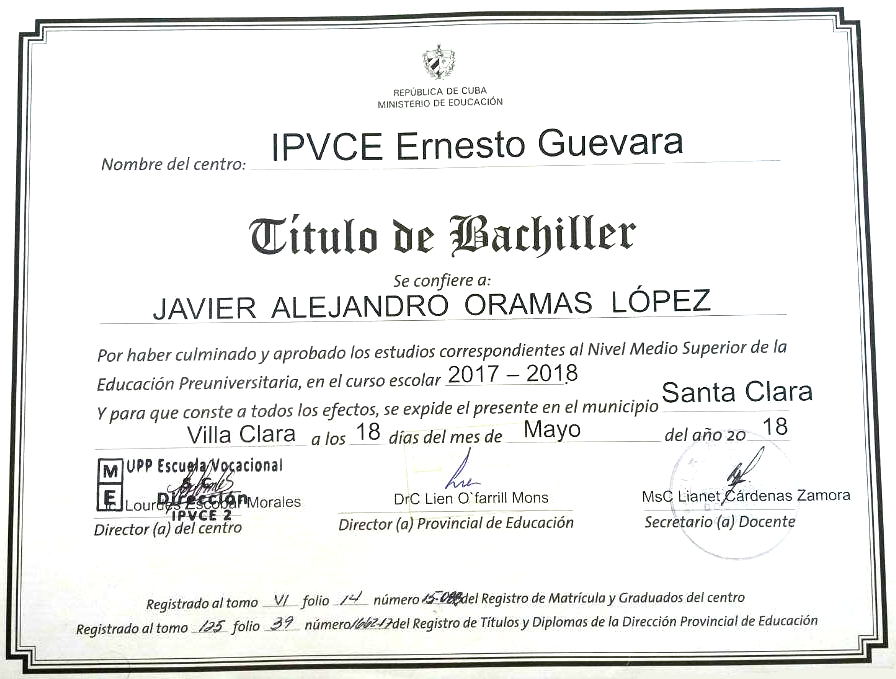
\includegraphics[width=\textwidth]{images/bachelor.png}
    \caption{Science Bachelor certificate}
    \label{sec:bachelor}
\end{figure}

\begin{figure}[h]
    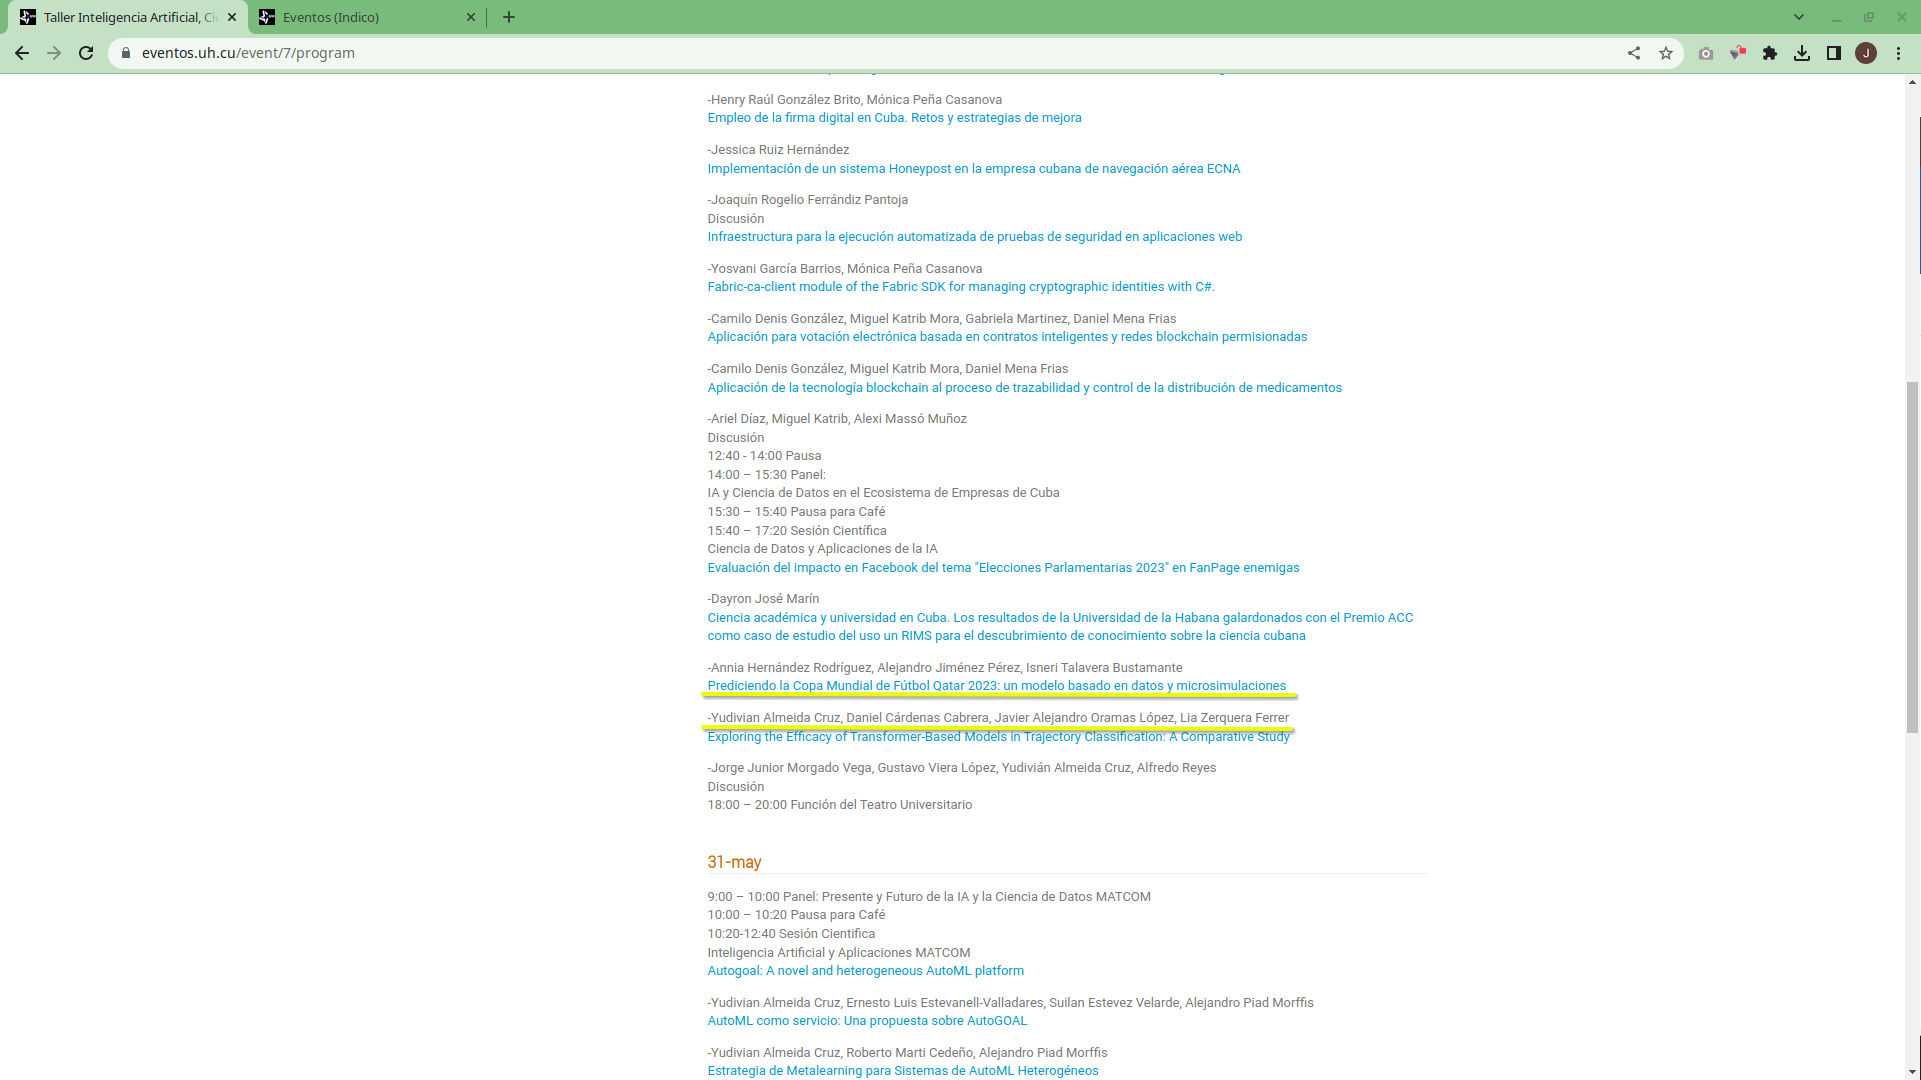
\includegraphics[width=\textwidth]{images/ai_workshop.png}
    \caption{\href{https://eventos.uh.cu/event/7/program}{Havana University events webpage}, screenshot 06/01/2023}
    \label{sec:workshop}
\end{figure}

\begin{figure}[h]
    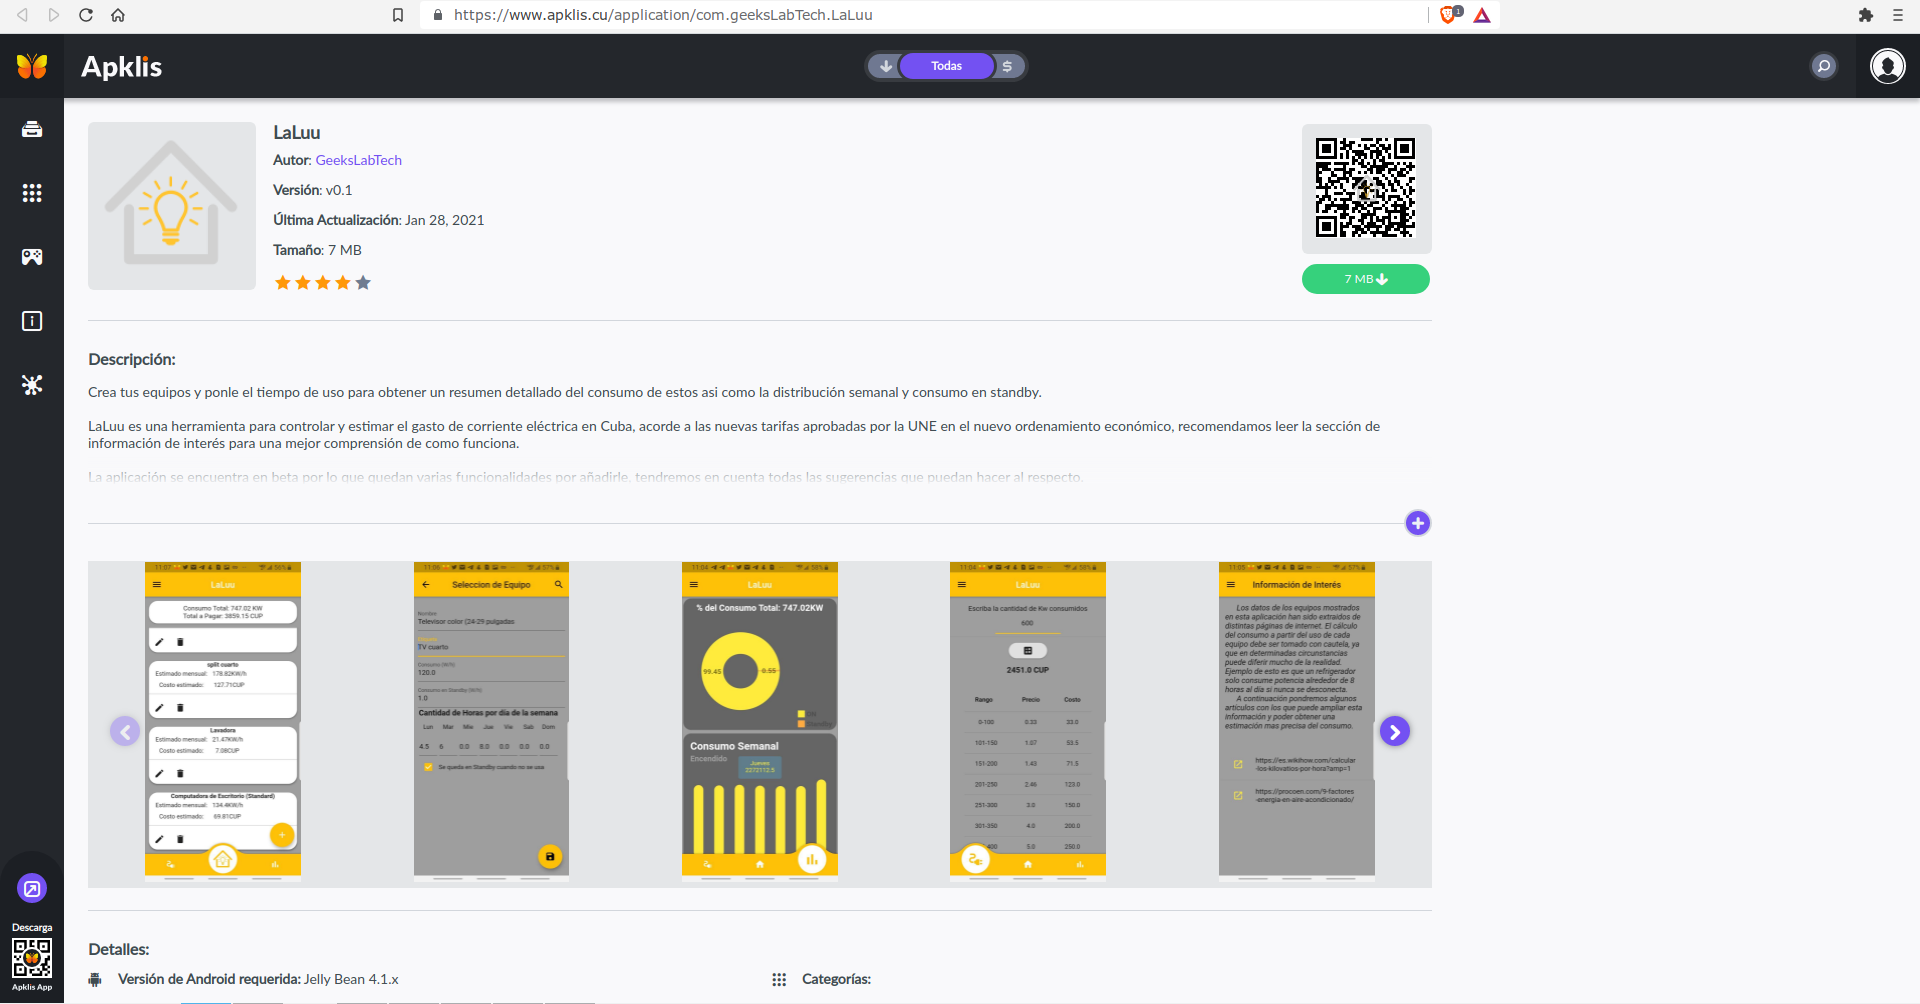
\includegraphics[width=\textwidth]{images/laluu.png}
    \caption{LaLuu app for estimation of Energy consumption. Available in \href{https://www.apklis.cu/application/com.geeksLabTech.LaLuu}{Apklis}, Cuban android app store, screenshot 01/25/2022}
    \label{sec:laluu}
\end{figure}

\begin{figure}[h]
    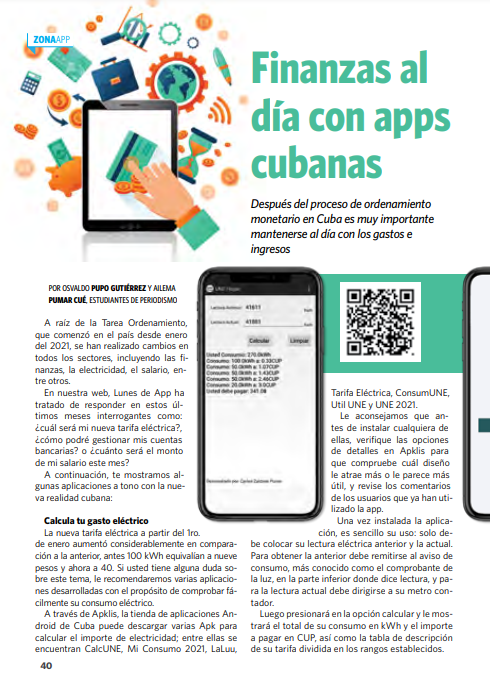
\includegraphics[width=\textwidth]{images/laluu_jt.png}
    \caption{Pupo, Gutiérrez O. y Pumar, Cué A. (may-jun 2021). \href{http://www.juventudtecnica.cu/sites/default/files/jt_420.pdf}{Finanzas al día con apps cubanas}. Juventud Técnica 420 (40-41), ISSN: 0449-4555, screenshot 01/25/2022}
    \label{sec:laluu_press}
\end{figure}

\begin{figure}[h]
    
\includegraphics[width=\textwidth]{images/laluu_art.png}
    \caption{Red Artemisa (february 2nd 2021).\href{https://www.artemisa.gob.cu/es/actualidad/noticias/9806-llego-febrero-calcula-tu-gasto-electrico-con-esta-apps}{Llegó febrero: calcula tu gasto eléctrico con esta apps.}, screenshot 01/25/2022}
\end{figure}

\begin{figure}[h]
    \includegraphics[width=\textwidth]{images/covid_19.png}
    \caption{\href{https://github.com/covid19cuba/covid19cuba-action}{Covid19CubaData app COVID-19 data analisys in Cuba}, screenshot 01/25/2022}
    \label{sec:covid}
\end{figure}

\begin{figure}[h]
    \includegraphics[width=\textwidth]{images/dengue.png}
    \caption{Competition Predicting Dengue Cases based on metheorological variables, using Machine Learning and Deep Learning. \href{https://www.drivendata.org/competitions/44/dengai-predicting-disease-spread}{DrivenData}, screenshot 01/25/2022}
    \label{sec:dengue}
\end{figure}

\begin{figure}[h]
    \includegraphics[width=\textwidth]{images/pythonpizza.png}
    \caption{Oramas, J. \href{https://holguin.python.pizza/?ref=python.pizza}{[Python Pizza Holguín]}. (nov 15th 2020). Video-Diet: poniendo a dieta tu almacenamiento \href{https://youtu.be/c--NOwM5W-0}{[Video]}.screenshot 01/25/2022}
    \label{sec:pythonpizza}
\end{figure}

\begin{figure}[h]
    \centering
    \includegraphics[height=0.8\textheight]{images/panamerican.png}
    \caption{\href{http://www.postdata.club/issues/201907/el-medallero-de-lima-2019-que-se-puede-esperar.html}{Almeida, Y. , Reyes, S. y Guerra, E. (jul 28th 2019). El medallero de Lima 2019 ¿qué podemos esperar? PostData.club Periodismo de Datos.}, screenshot 01/25/2022}
    \label{sec:panamerican}
\end{figure}

\begin{figure}[h]
    \centering
    \includegraphics[width=\textwidth]{images/icpckej.png}
    \caption{ \href{https://icpc.global/regionals/finder/cnc-2018/standings}{International Collegiate Programming Contest (oct 2018). Standings for The 2018 ACM-ICPC Caribbean National Contests}. screenshot 01/25/2022}
    \label{sec:icpc_kej}
\end{figure}

\begin{figure}[h]
    \centering
    \includegraphics[width=\textwidth]{images/icpckej_standing.png}
    \caption{\href{https://matcomgrader.com/post/5179/resultados-del-concurso-local-caribeno-2018}{Matcom Online Grader (sept 2018). Resultados del Concurso Local Caribeño 2018. Facultad de Matemática y Ciencia de la Computación, Universidad de La Habana.}, screenshot 01/25/2022}
    % \label{sec:}
\end{figure}

\begin{figure}[h]
    \centering
    \includegraphics[width=\textwidth]{images/letter.png}
    \caption{General Director invitation letter, Caribbean Finals ACM - ICPC 2017, screenshot 01/25/2022}
    \label{sec:letter}
\end{figure}

\begin{figure}[h]
    \centering
    \includegraphics[width=\textwidth]{images/team3c.jpg}
    \caption{\href{https://matcomgrader.com/post/5167/the-2017-acm-icpc-caribbean-finals}{Matcom Online Grader (oct 2017). The 2017 ACM-ICPC Caribbean Finals. Facultad de Matem?tica y Ciencia de la Computaci?n, Universidad de La Habana} screenshot 01/25/2022}
    \label{sec:3c}
\end{figure}
\begin{figure}[h]
    \centering
    \includegraphics[width=\textwidth]{images/icpc_classified.png}
    \caption{\href{ https://coj-forum.uci.cu/viewtopic.php?t=3315}{Caribbean Online Judge (nov 2017). Final Caribe?a del ACM - ICPC 2017.}, screenshot 01/25/2022}
    \label{sec:icpc}
\end{figure}

\begin{figure}[h]
    \centering
    \includegraphics[width=\textwidth]{images/2017final.png}
    \caption{Participation Certificate, ACM-ICPC 2017 Cuban Finals, screenshot 01/25/2022}
    \label{sec:2017final}
\end{figure}


\begin{figure}[h]
    \centering
    \includegraphics[width=\textwidth]{images/uclv_cup.png}
    \caption{Participation Certificate, IV Programming Cup, Universidad Central de Las Villas, screenshot 01/25/2022}
    \label{sec:uclv_cup}
\end{figure}


\begin{figure}[h]
    \centering
    \includegraphics[width=\textwidth]{images/nac_contest.png}
    \caption{Certificate for Relevant Results obtained in the National Informatics Competition, Mach 2017, screenshot 01/25/2022}
    \label{sec:nac_contest}
\end{figure}


\begin{figure}[h]
    \centering
    \includegraphics[width=\textwidth]{images/ibero.png}
    \caption{Certificate of Participation, Iberoamerican Computer Correspondence Competition, México 2016, screenshot 01/25/2022}
    \label{sec:}
\end{figure}


\begin{figure}[h]
    \centering
    \includegraphics[width=\textwidth]{images/preseleccion.png}
    \caption{Certificate from the Ministry of Education of Cuba for having integrated the National Preselection to the International Olympiads of Informatics. 2016, screenshot 01/25/2022}
    \label{sec:preseleccion}
\end{figure}


\begin{figure}[h]
    \centering
    \includegraphics[width=\textwidth]{images/tinajon.png}
    \caption{Certificate for Third place obtained in the Regional Cup of Computer Science Competition, Camag\"uey December 2015, screenshot 01/25/2022}
    \label{sec:tinajon}
\end{figure}


\begin{figure}[h]
    \centering
    \includegraphics[width=\textwidth]{images/2016nacional.png}
    \caption{Certificate of participation in the National Competition of the ACM-ICPC, Universidad Central de Las Villas, October 2015, screenshot 01/25/2022}
    \label{sec:nacional2016}
\end{figure}


\begin{figure}[h]
    \centering
    \includegraphics[width=\textwidth]{images/2016local.png}
    \caption{Certificate of participation in the Local Competition of the ACM-ICPC, Universidad Central de Las Villas, September 2015, screenshot 01/25/2022}
    \label{sec:local2016}
\end{figure}

\begin{figure}[h]
    \centering
    \includegraphics[width=\textwidth]{images/informatica.png}
    \caption{Recognition for second place obtained in the National Computer Science Competition, Marzo 2014, screenshot 01/25/2022}
    \label{sec:informatic}
\end{figure}

\end{document}
